%!TEX root = main.tex

\chapter{Insights on Grover Search Algorithm and its implementation}
\label{chp:grover}

\section{Introduction}

\subsection{Premise}

Many quantum algorithms base their reason to exist in the fact that a small routine of the them (e.g. the search for the next arc to be considered among those coming out of a given node, in Max Flow Analysis) is done by a quantum computer. It is usually nothing more than a search in a list (or more generally in a database) of one or more elements that satisfy a certain condition (the arcs that have not been visited yet, i.e. having infinite weight value).

\subsection{The problem}

Let's start noticing that although we have presented in \cref{sec:QSgrover} an implementation of Grover Search in Q\#, it actually works on what is known as ``virtual database''. Alike real databases, virtual (or implicit) ones are not really databases: given $n$ as the number of bits, they are nothing more than the set of integer numbers $\left[0, 2^{n-1}\right]$.

Such a ``database'' can be easily implemented with a quantum register initialized with $H^{\oplus n}$. In this way, whenever the register is measured, it collapses to one of all the possible combinations of its bits (i.e. $\left[0, 2^{n-1}\right]$), being all these combinations all equally probable.

\bigskip

Actually the implementation described in \cref{sec:QSgrover} complies with most of the available literature \cite{Grover:1996:FQM:237814.237866, lavor2003grover}. It is evident that currently most of the works someway related to Grover Search Algorithm are devoted to quantum search on virtual databases. \cite{Broda2016}

\bigskip

Apparently some people agree that Grover is limited to implicit databases, therefore not convenient or even not useful at all for real databases \cite{1425397, Zalka2000, stackexchange1, stackexchange2, stackexchange3}. On the other hand, someone had a deeper study on the algorithm, understanding the mechanism and implementing (at least mathematically) the encoding and the search on a real database. \cite{alsing2011grover}

%\bigskip
%
%We will build on this last paper to answer the questions:
%\begin{itemize}
%	\item Is it correct to use Grover Search for a real database search?
%	\item Is it feasible? (i.e. could an algorithm be devised to do so?)
%\end{itemize}

%TODO an outline of this chapter

\section{The phone book implementation}

The work \cite{alsing2011grover} actually finds a way to encode some elements into a real database. It is done setting a register to an entangled state, as sum of the states corresponding to the elements that we want to encode into the database. This database-register is created by applying a particular matrix to it, in which the database elements are encoded within the rows order. An example is shown in \cref{fig:row_swap}.

\begin{figure}
	\centering
	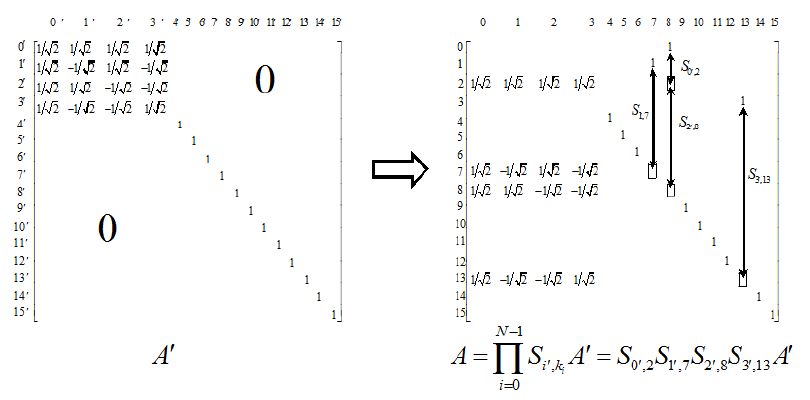
\includegraphics[width=\linewidth]{row_swap}
	\caption{Successive row swapping operations to transform $A'$ to $A$ in for the specific telephone database example. (credits to \cite{alsing2011grover})}
	\label{fig:row_swap}
\end{figure}

Calling $n$ the number of bits of the primary key (i.e. the contact \textit{name}) and $m$ the number of bits of the data field (i.e. the contact \textit{number}), the square matrix $A'$ will have a size of $K = 2^n \cdot 2^m = 2^{n+m}$ rows. Matrix $A'$ can be obtained as a direct sum $H^{\otimes n} \oplus I_{K-2^n}$ (see \cref{sec:direct_sum}).

Matrix $A$ can be obtained by applying to $A'$ a series of swap operators $S_{ij}$ that perform a swapping between rows $i$ and $j$ of a matrix. This operation is not described in the proposed paper, therefore we will try to give an algorithm to perform it (see \cref{sec:permutation}). This is the key passage that let us prepare an entangled register, ready to be used for the subsequent Grover iterations, as shown in the mentioned work.

\bigskip

This is a remarkable result, as it demonstrates the theoretical consistency of Grover's Algorithm for searching purposes. Critics can be raised against the performance or the convenience of the entire process with respect to the classical one, but these topics have already been discussed elsewhere \cite{1425397}.

\section{Permutation of rows in a matrix}
\label{sec:permutation}

The main issue that we want to address now is how to perform an arbitrary permutation of the rows of a ``quantum'' matrix. This is a fundamental algorithm passage for the correct implementation of Grover iteration. Despite that, we were not able to find any hint in literature on how to perform such permutations, so here we present some ideas that can be a starting point for a future improved and more general solution of the problem.

\bigskip

As it is well known in linear algebra, given a square matrix $M$ we can obtain $M'$ (a version of it where $i$-th and $j$-th rows are swapped) multiplying $M$ by a matrix $E$, where $E$ is the identity with $i$-th and $j$-th rows swapped:

\begin{equation*}
E M = M'
\end{equation*}
\begin{equation*}
	\begin{bmatrix}
	1 & 0 & 0 & 0\\
	0 & 1 & 0 & 0\\
	0 & 0 & 0 & 1\\
	0 & 0 & 1 & 0\\
	\end{bmatrix}
	\begin{bmatrix}
	a_{11} & a_{12} & a_{13} & a_{14}\\
	a_{21} & a_{22} & a_{23} & a_{24}\\
	a_{31} & a_{32} & a_{33} & a_{34}\\
	a_{41} & a_{42} & a_{43} & a_{44}\\
	\end{bmatrix}
	=
	\begin{bmatrix}
	a_{11} & a_{12} & a_{13} & a_{14}\\
	a_{21} & a_{22} & a_{23} & a_{24}\\
	a_{41} & a_{42} & a_{43} & a_{44}\\
	a_{31} & a_{32} & a_{33} & a_{34}\\
	\end{bmatrix}
\end{equation*}

\bigskip

Therefore our problem is to find a circuit that implements matrix $E$. This technique is consistent with the fact that a circuit applied on an array of qubit can be represented with a matrix multiplying the vector from the left side. Multiplying $E$ from the left of $M$ is equivalent to placing the circuit of $E$ after (on the right of) the circuit of $M$.

\begin{equation*}
\Qcircuit @R=1.0em @!R {
	\lstick{b_{0}: } & \multigate{2}{M}	& \multigate{2}{E}	& \qw \\
	\lstick{b_{1}: } & \ghost{M}		& \ghost{E}			& \qw \\
	\lstick{b_{2}: } & \ghost{M}		& \ghost{E}			& \qw \\
}
\end{equation*}

\subsection{Simplified case: 2 qubits}

If we have a circuit of only 2 qubits, swapping 2 rows can be relatively easy.

\bigskip

\noindent
\begin{tabular} {m{0.3\linewidth} m{0.7\linewidth}}
	\hline
	Rows to swap	& Matrices to apply\\
	\hline
	1, 2	&	ICNOT (\textit{NOT gate} controlled on first qubit = 0)\\
	1, 3	&	SWAP $\cdot$ ICNOT $\cdot$ SWAP\\
	1, 4	&	CNOT $\cdot$ SWAP $\cdot$ ICNOT $\cdot$ SWAP $\cdot$ CNOT\\
	2, 3	&	SWAP\\
	2, 4	&	CNOT $\cdot$ SWAP $\cdot$ CNOT\\
	3, 4	&	CNOT\\
	\hline
\end{tabular}

\bigskip

For example:

\begin{equation*}
CNOT \cdot SWAP \cdot CNOT = swap(2,4)
\end{equation*}
\begin{equation*}
\Qcircuit @R=1em @!R {
	\lstick{} & \ctrl{1}	& \qswap		& \ctrl{1}	& \qw \\
	\lstick{} & \targ	& \qswap \qwx	& \targ		& \qw \\
}
\end{equation*}

\begin{equation*}
\begin{bmatrix}
1 & 0 & 0 & 0 \\
0 & 1 & 0 & 0 \\
0 & 0 & 0 & 1 \\
0 & 0 & 1 & 0 \\
\end{bmatrix}
\begin{bmatrix}
1 & 0 & 0 & 0 \\
0 & 0 & 1 & 0 \\
0 & 1 & 0 & 0 \\
0 & 0 & 0 & 1 \\
\end{bmatrix}
\begin{bmatrix}
1 & 0 & 0 & 0 \\
0 & 1 & 0 & 0 \\
0 & 0 & 0 & 1 \\
0 & 0 & 1 & 0 \\
\end{bmatrix}
=
\begin{bmatrix}
1 & 0 & 0 & 0 \\
0 & 0 & 0 & 1 \\
0 & 0 & 1 & 0 \\
0 & 1 & 0 & 0 \\
\end{bmatrix}
\end{equation*}

\subsection{General case: shift and control}

A possible extension of the algorithm to the case of $n$ qubits would make an intensive use of controlled gates. Control through a qubit equal to 1 is equivalent to the direct sum of an identity matrix and the controlled gate itself. This means that, if we can control a gate, we are able to replicate the behavior of its $4 \times 4$ matrix in the bottom half of a larger $8 \times 8$ matrix (in terms of rows swapping). It could be interesting if we could temporarily ``move down'' the rows of a big matrix, perform our swaps and then move them up again. To easier describe this process we will make some definitions.

\bigskip

\textit{Definition.} Let $N$ denote the number of rows in the matrix representing an operation $G$. The number $N$ is obviously $2^n$, where $n$ is the number of bits on which gate $G$ is applied. Let's consider only a gate G which is decomposable as a direct product of a matrix $M$ and an identity matrix $I_k$. We will call $k$ the \textit{grade} of operator $G$.

\bigskip

Example:
\begin{itemize}
	\item CNOT and SWAP have \textit{grade} 0
	\item CNOT3, SWAP3 and SHIFT3 (\cref{sec:derived_gates}) have \textit{grade} 1
	\item SHIFT4 (\cref{sec:derived_gates}) has \textit{grade} 2
	\item CCNOT has grade 0
\end{itemize}

We can easily increase by $h$ the degree of a matrix $G$ by performing $kron(G, I_h)$. This is equivalent, in a register large $n+h$ qubits, to apply $G$ to the first $n$ qubits and nothing to the remaining $h$.

\subsubsection{Algorithm}

Let's take as an example the problem of permuting rows of an $8 \times 8$ matrix.

Using CNOT3, SWAP3 and ICNOT3 we can exchange matrix macroblocks (blocks of 2 contiguous lines). We can then operate on the two blocks (each 2x8) of the lower half-matrix using the CCNOT, CSWAP and controlled ICNOT ports, with granularity of the individual rows. Please note that the CSWAP allows us to exchange two rows of two different blocks (2x8), this can be useful in the generalization to more qubits. The same algorithm can be used for 16x16 matrices, increasing by one the degree of all previous ports and adding one more bit of control to the existing port (thus obtaining CCCNOT, CCICNOT, CCSWAP...).

Useful gates to perform the shift are SHIFT, QSD and QSU gates, together with their higher grade versions (\cref{sec:derived_gates}).

\subsubsection{Open issues}

Probably the addition of new control qubits at each step of generalization implies an exponential growth in spatial complexity of the circuit.

\subsection{General case: sorting algorithms}

This approach, instead of focusing on single row swaps, treats the permutation from initial to final matrix as a single process. You can see the analogy with sorting algorithms applied to arrays (bubble sort, merge sort...).

If there was a way to swap 2 consecutive rows of a matrix, regardless of their position, the problem would be easily solved. In that case we could apply bubble sort as an algorithm to rearrange all the rows as we like.

\bigskip

The only general way that we could devise to exchange consecutive rows is to use $X$ gates in direct sum with $I_2$ matrices all over the diagonal. The main drawback of this method is that this configuration is only able to swap rows $2i+1$ and $2i+2$, with $i \geq 0$. Therefore if we want to swap for example rows 2 and 3 we need to use a SWAP gate in direct sum with an appropriate number of $I$ matrices down the diagonal. The problem in using SWAP in this configuration is that it works only for swapping rows $4i+2$ and $4i+3$, with $i \geq 0$. Therefore if we want to swap rows 4 and 5 we need a new different gate (possibly $8 \times 8$ or bigger) and so on.

%\section{Feasibility analysis}

%TODO